\subsection{Coupled ODE--CTMC systems}
\label{m:sec:coupled}

The chains of \cref{m:sec:ctmc,m:sec:inhomog} have rates that are either fixed
numbers or prescribed functions of time. Several later chapters need a third
possibility: rates that are functions of quantities evolving according to their
own deterministic dynamics, where those dynamics in turn depend on the state of
the chain. This section fixes the framework for such systems. It is conceptual
--- the framework and one schematic example --- and the concrete models built on
it are developed \fwd{rupture}{in the later chapters on compartment rupture and
shared media}.

\subsubsection{The framework}
\label{m:sec:coupledframe}

Let the state of the system be a pair $(Y_t,X_t)$, where $X_t$ is a CTMC on a
countable state space $\mathcal S$, interpreted as the discrete configuration
of a population or of a collection of compartments, and $Y_t\in\mathbb R^d$ is
a vector of continuous variables --- concentrations, accumulated damage, the
contents of a shared medium. The coupling has two directions.

\begin{definition}[Coupled ODE--CTMC system]
\label{m:def:coupled}
Between jumps of $X$, the continuous state evolves by
\begin{equation}
\label{m:eq:coupledode}
\dda{Y}{t} = f(Y_t,X_t),
\end{equation}
with $f:\mathbb R^d\times\mathcal S\to\mathbb R^d$. When $X_t=i$, the chain
jumps to $j$ at rate $q_{ij}(Y_t)$, so that the generator depends on the current
continuous state:
\begin{equation}
\label{m:eq:coupledrates}
\pr{X_{t+\Delta t}=j\mid X_t=i,\ Y_t} = q_{ij}(Y_t)\,\Delta t + o(\Delta t).
\end{equation}
The dependence may operate in either direction alone, or in both at once.
\end{definition}

The joint process $(Y_t,X_t)$ is Markov whenever the ODE flow is well posed ---
say $f(\cdot,i)$ locally Lipschitz for each $i$ --- and the rates are
measurable and bounded on bounded sets. It belongs to the class of
\emph{piecewise-deterministic Markov processes}: the randomness enters only
through the jump mechanism, and between jumps the trajectory is a solution of an
ordinary differential equation \cite{Davis1993}. Two limiting cases connect the
definition to earlier material. If $q_{ij}$ does not actually depend on $Y$,
\cref{m:def:coupled} reduces to a CTMC forcing an ODE; if $f$ does not depend on
$X$, it reduces to an ODE whose coefficients are modulated by an external chain.
The genuinely coupled case, which is the one that appears in this thesis, uses
both dependences at once (\cref{m:fig:coupled}).

\begin{figure}[ht]
\centering
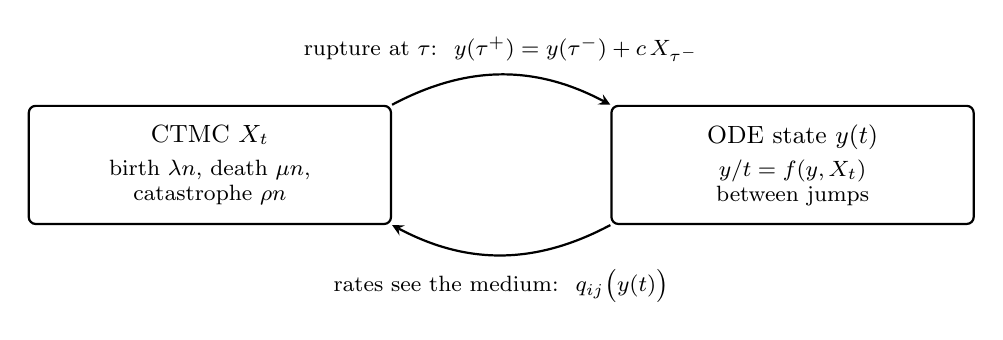
\begin{tikzpicture}[
    box/.style={draw, thick, rounded corners=2.5pt, minimum width=4.6cm,
                minimum height=1.5cm, align=center, font=\small},
    arr/.style={-stealth, thick},
    lab/.style={font=\footnotesize, align=center}
]
\node[box] (ctmc) at (0,0) {CTMC $X_t$\\[1pt]
  {\footnotesize birth $\lambda n$, death $\mu n$,}\\[-2pt]
  {\footnotesize catastrophe $\rho n$}};
\node[box] (ode) at (7.4,0) {ODE state $y(t)$\\[1pt]
  {\footnotesize $\dd y/\dd t = f(y,X_t)$}\\[-2pt]
  {\footnotesize between jumps}};
\draw[arr] (ctmc.north east) to[bend left=28]
  node[lab, above=1pt] {rupture at $\tau$:\; $y(\tau^+) = y(\tau^-) + c\,X_{\tau^-}$}
  (ode.north west);
\draw[arr] (ode.south west) to[bend left=28]
  node[lab, below=1pt] {rates see the medium:\; $q_{ij}\bigl(y(t)\bigr)$}
  (ctmc.south east);
\end{tikzpicture}
\caption{The two directions of the coupling in \cref{m:def:coupled}. The jump
process $X_t$ drives the flow through its state (and, at a rupture, through an
impulsive release into the medium), while the continuous state $y(t)$ modulates
the transition rates of the chain. Between jumps the trajectory is a solution of
an ODE; randomness enters only at the jumps, which is the
piecewise-deterministic structure of \cite{Davis1993}.}
\label{m:fig:coupled}
\end{figure}

The one-way versions are familiar in the applications. A chain forcing an ODE
is what one obtains when discrete events feed a continuous reservoir: each jump
of $X$ changes the source term of \cref{m:eq:coupledode}, and the reservoir
integrates the resulting forcing between jumps. An ODE modulating a chain is the
natural description of an environment: a drug concentration that decays
deterministically while the per-capita death rate of a population is a function
of it.

\subsubsection{Simulation and analysis}
\label{m:sec:coupledsim}

The construction of \cref{m:prop:race} extends to \cref{m:def:coupled} with one
qualification: the rates are no longer constant between events, because $Y_t$
moves. Given the current state $(Y,i)$, integrate \cref{m:eq:coupledode} with
$X\equiv i$ to obtain $Y_s$ for $s\ge t$; the total jump rate
$q_i(Y_s)=\sum_jq_{ij}(Y_s)$ is then a known function of $s$, and the next jump
time $T$ has survival function
\begin{equation*}
\pr{T>s} = \exp\lrb{-\int_t^{s}q_i(Y_u)\,\dd u},
\end{equation*}
exactly as in \cref{m:sec:timedep}; the jump destination is drawn with
probability $q_{ij}(Y_T)/q_i(Y_T)$, the state is updated, and the procedure
repeats. When $q_i$ is bounded, the integral can be inverted by rejection on a
constant majorant; otherwise it is quadrature, and the scheme is the standard
event-driven simulator for piecewise-deterministic processes.

Analytically, two routes are available. If the coupling is weak, one replaces
$Y_t$ by its mean-field trajectory, obtaining a time-inhomogeneous chain in the
sense of \cref{m:sec:inhomog} --- the logistic speciation model of
\cref{m:sec:logspec} is precisely that closure --- or replaces $X_t$ by its
mean, obtaining a closed ODE. When the coupling is strong neither closure is
exact, and the working objects are the joint expectations, which satisfy hybrid
moment equations mixing the generator of the chain with the drift $f$; those are
developed as needed \fwd{rupture}{in the chapters on rupture and shared media}.

\subsubsection{A schematic example: rupture feeding a shared medium}
\label{m:sec:coupledexample}

The example that organises the later chapters is a compartment that can rupture
into a shared medium. Let $X_t$ be the contents of the compartment, evolving as
the birth--death--catastrophe process of \cref{m:def:bdc}, and let $y(t)\ge0$
be the concentration of material in the shared medium. Between ruptures the
medium loses material at rate $\delta$,
\begin{equation*}
\dda{y}{t} = -\delta y ,
\end{equation*}
and at the rupture time $\tau$ the entire contents of the compartment are
released into the medium in one jump,
\begin{equation*}
y(\tau+) = y(\tau-) + c\,X_{\tau-} .
\end{equation*}
The reverse direction of the coupling is equally present: the absorption rate at
which surviving compartments take up material from the medium, and the
catastrophe rate $\rho$ itself, may both be functions of the current
concentration $y(t)$, so that a fuller medium accelerates uptake and can
destabilise what remains. Written in the notation of \cref{m:def:coupled}, this
is a system in which $f$ depends on $X$ (release occurs only through the
catastrophe channel) and $q_{ij}$ depends on $Y$ (the rates see the medium), so
both arrows of the definition are active.

Two features of this schematic are worth isolating, because they recur in every
instantiation of it. The ODE variable $y$ is \emph{impulsive}: it evolves
smoothly between jumps and discontinuously at them, so its natural description
is a flow plus jump maps rather than a single differential equation. And the
quantity released at rupture, $X_{\tau-}$, is the state of the chain at a
stopping time, not a parameter: the rupture cohort is whatever the catastrophe
finds, and its distribution is the quasi-stationary-type problem of
\cref{m:sec:methct} evaluated at a random time. Both features are why the
models built on \cref{m:def:coupled} are analysed with generating-function and
first-step machinery rather than closed by simulation alone.

\begin{figure}[ht]
\centering

\includegraphics[width=0.92\textwidth]{figures/rupture_sawtooth.pdf}
\caption{A single exact event-driven realisation of the coupled rupture system
of \cref{m:sec:coupledexample}, with $\lambda=0.55$, $\mu=0.25$, $\rho=0.08$,
$N_0=5$, $\delta=0.30$ and $c=0.4$; for illustration the compartment is
re-seeded with $N_0$ individuals after each rupture. Top: the compartment
contents $X_t$, growing between ruptures and collapsing at them. Bottom: the
shared medium $y(t)$, decaying exponentially between ruptures and receiving the
impulsive release $c\,X_{\tau-}$ at each one; the jumps grow with the cohort
the catastrophe finds. Dotted vertical lines mark the rupture times, aligned
across the panels.}
\label{m:fig:sawtooth}
\end{figure}

\FloatBarrier
